% Options for packages loaded elsewhere
% Options for packages loaded elsewhere
\PassOptionsToPackage{unicode}{hyperref}
\PassOptionsToPackage{hyphens}{url}
\PassOptionsToPackage{dvipsnames,svgnames,x11names}{xcolor}
%
\documentclass[
]{article}
\usepackage{xcolor}
\usepackage[margin=1in]{geometry}
\usepackage{amsmath,amssymb}
\setcounter{secnumdepth}{-\maxdimen} % remove section numbering
\usepackage{iftex}
\ifPDFTeX
  \usepackage[T1]{fontenc}
  \usepackage[utf8]{inputenc}
  \usepackage{textcomp} % provide euro and other symbols
\else % if luatex or xetex
  \usepackage{unicode-math} % this also loads fontspec
  \defaultfontfeatures{Scale=MatchLowercase}
  \defaultfontfeatures[\rmfamily]{Ligatures=TeX,Scale=1}
\fi
\usepackage{lmodern}
\ifPDFTeX\else
  % xetex/luatex font selection
\fi
% Use upquote if available, for straight quotes in verbatim environments
\IfFileExists{upquote.sty}{\usepackage{upquote}}{}
\IfFileExists{microtype.sty}{% use microtype if available
  \usepackage[]{microtype}
  \UseMicrotypeSet[protrusion]{basicmath} % disable protrusion for tt fonts
}{}
\makeatletter
\@ifundefined{KOMAClassName}{% if non-KOMA class
  \IfFileExists{parskip.sty}{%
    \usepackage{parskip}
  }{% else
    \setlength{\parindent}{0pt}
    \setlength{\parskip}{6pt plus 2pt minus 1pt}}
}{% if KOMA class
  \KOMAoptions{parskip=half}}
\makeatother
% Make \paragraph and \subparagraph free-standing
\makeatletter
\ifx\paragraph\undefined\else
  \let\oldparagraph\paragraph
  \renewcommand{\paragraph}{
    \@ifstar
      \xxxParagraphStar
      \xxxParagraphNoStar
  }
  \newcommand{\xxxParagraphStar}[1]{\oldparagraph*{#1}\mbox{}}
  \newcommand{\xxxParagraphNoStar}[1]{\oldparagraph{#1}\mbox{}}
\fi
\ifx\subparagraph\undefined\else
  \let\oldsubparagraph\subparagraph
  \renewcommand{\subparagraph}{
    \@ifstar
      \xxxSubParagraphStar
      \xxxSubParagraphNoStar
  }
  \newcommand{\xxxSubParagraphStar}[1]{\oldsubparagraph*{#1}\mbox{}}
  \newcommand{\xxxSubParagraphNoStar}[1]{\oldsubparagraph{#1}\mbox{}}
\fi
\makeatother


\usepackage{longtable,booktabs,array}
\newcounter{none} % for unnumbered tables
\usepackage{calc} % for calculating minipage widths
% Correct order of tables after \paragraph or \subparagraph
\usepackage{etoolbox}
\makeatletter
\patchcmd\longtable{\par}{\if@noskipsec\mbox{}\fi\par}{}{}
\makeatother
% Allow footnotes in longtable head/foot
\IfFileExists{footnotehyper.sty}{\usepackage{footnotehyper}}{\usepackage{footnote}}
\makesavenoteenv{longtable}
\usepackage{graphicx}
\makeatletter
\newsavebox\pandoc@box
\newcommand*\pandocbounded[1]{% scales image to fit in text height/width
  \sbox\pandoc@box{#1}%
  \Gscale@div\@tempa{\textheight}{\dimexpr\ht\pandoc@box+\dp\pandoc@box\relax}%
  \Gscale@div\@tempb{\linewidth}{\wd\pandoc@box}%
  \ifdim\@tempb\p@<\@tempa\p@\let\@tempa\@tempb\fi% select the smaller of both
  \ifdim\@tempa\p@<\p@\scalebox{\@tempa}{\usebox\pandoc@box}%
  \else\usebox{\pandoc@box}%
  \fi%
}
% Set default figure placement to htbp
\def\fps@figure{htbp}
\makeatother





\setlength{\emergencystretch}{3em} % prevent overfull lines

\providecommand{\tightlist}{%
  \setlength{\itemsep}{0pt}\setlength{\parskip}{0pt}}



 


\usepackage{lineno}
\linenumbers
\usepackage{float}
\usepackage[font=small,labelfont=bf]{caption}
\makeatletter
\@ifpackageloaded{caption}{}{\usepackage{caption}}
\AtBeginDocument{%
\ifdefined\contentsname
  \renewcommand*\contentsname{Table of contents}
\else
  \newcommand\contentsname{Table of contents}
\fi
\ifdefined\listfigurename
  \renewcommand*\listfigurename{List of Figures}
\else
  \newcommand\listfigurename{List of Figures}
\fi
\ifdefined\listtablename
  \renewcommand*\listtablename{List of Tables}
\else
  \newcommand\listtablename{List of Tables}
\fi
\ifdefined\figurename
  \renewcommand*\figurename{Figure}
\else
  \newcommand\figurename{Figure}
\fi
\ifdefined\tablename
  \renewcommand*\tablename{Table}
\else
  \newcommand\tablename{Table}
\fi
}
\@ifpackageloaded{float}{}{\usepackage{float}}
\floatstyle{ruled}
\@ifundefined{c@chapter}{\newfloat{codelisting}{h}{lop}}{\newfloat{codelisting}{h}{lop}[chapter]}
\floatname{codelisting}{Listing}
\newcommand*\listoflistings{\listof{codelisting}{List of Listings}}
\makeatother
\makeatletter
\makeatother
\makeatletter
\@ifpackageloaded{caption}{}{\usepackage{caption}}
\@ifpackageloaded{subcaption}{}{\usepackage{subcaption}}
\makeatother
\usepackage{bookmark}
\IfFileExists{xurl.sty}{\usepackage{xurl}}{} % add URL line breaks if available
\urlstyle{same}
\hypersetup{
  pdftitle={Supplementary Information},
  colorlinks=true,
  linkcolor={blue},
  filecolor={Maroon},
  citecolor={Blue},
  urlcolor={Blue},
  pdfcreator={LaTeX via pandoc}}


\title{Supplementary Information}
\usepackage{etoolbox}
\makeatletter
\providecommand{\subtitle}[1]{% add subtitle to \maketitle
  \apptocmd{\@title}{\par {\large #1 \par}}{}{}
}
\makeatother
\subtitle{The metabolic cost of the febrile host across the priority
Candida}
\author{}
\date{}
\begin{document}
\maketitle


\section{Supplementary figures}\label{supplementary-figures}

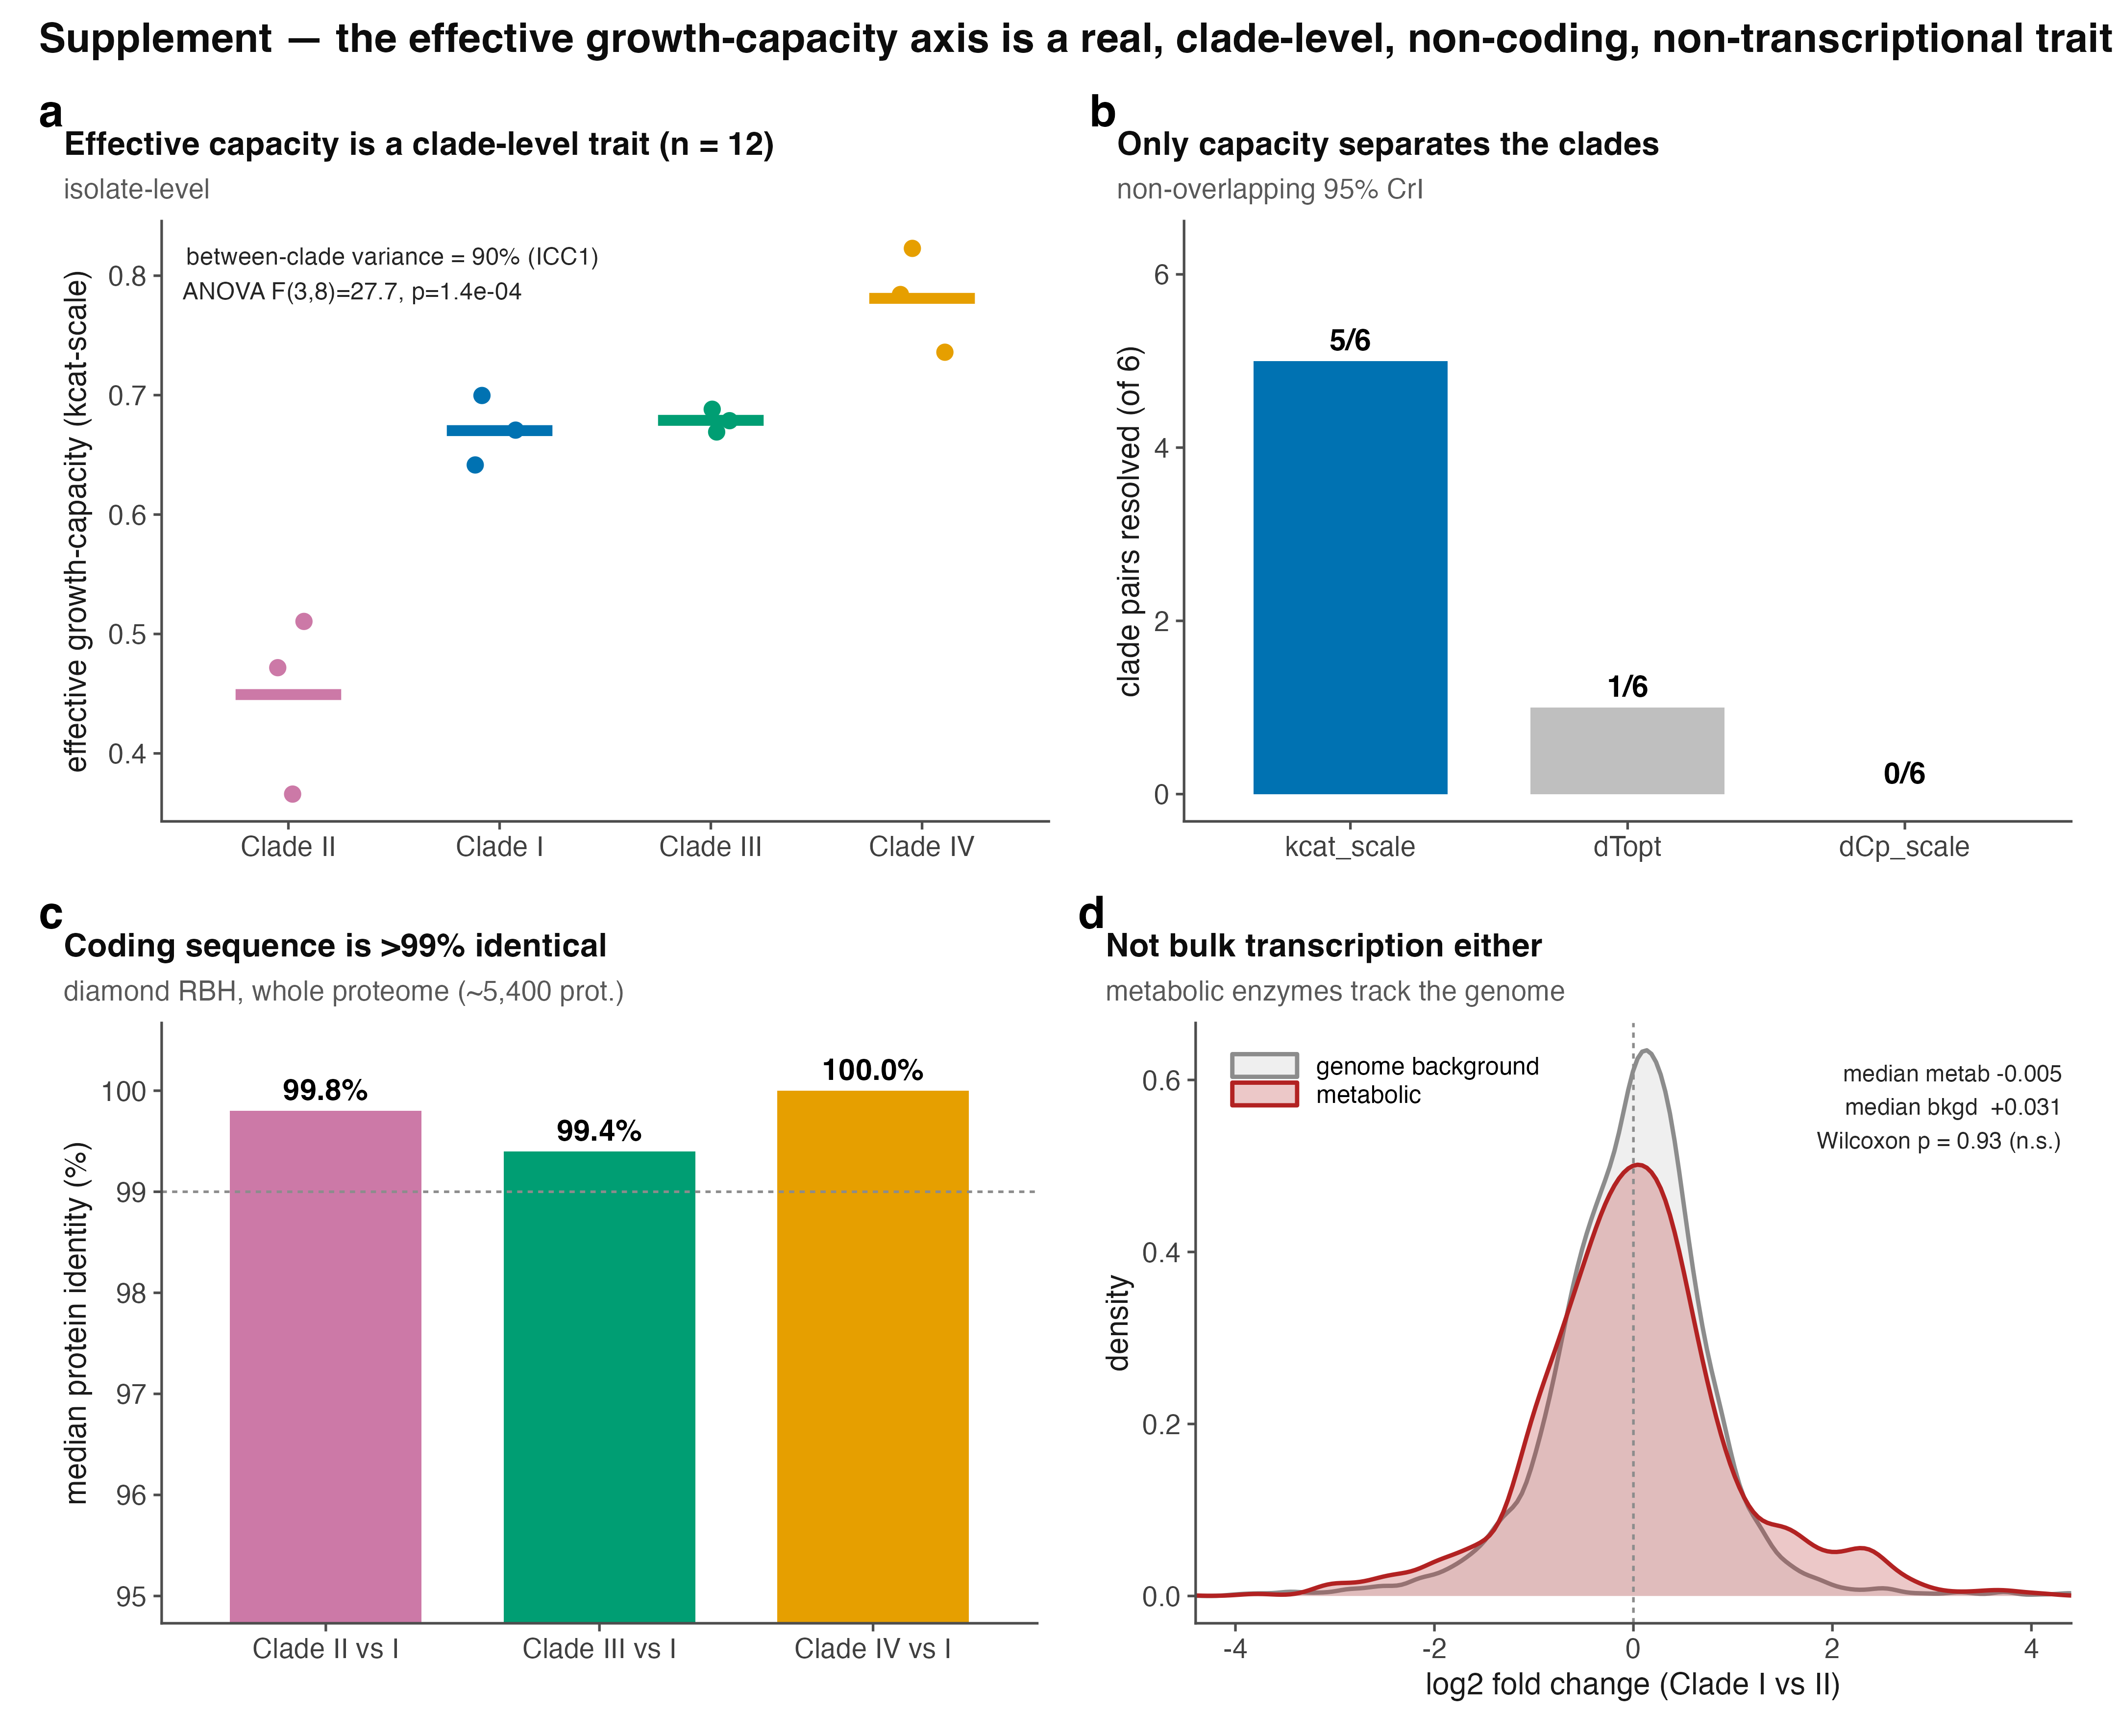
\includegraphics[width=1\linewidth,height=\textheight,keepaspectratio]{../../results/figures/manuscript/FIG_MODEL_SUPP_validation.png}

\textbf{Supplementary Figure 1. The effective growth-capacity axis is a
real, clade-level, non-coding, non-transcriptional trait.} (\textbf{a})
Capacity across the twelve isolates by clade (bars, clade means); 90\%
of the variance lies between clades (ICC\textsubscript{1} = 0.90).
(\textbf{b}) Number of clade pairs resolved (non-overlapping 95\% CrI)
by each calibration parameter; only the effective growth-capacity
parameter (kcat-scale) separates the clades. (\textbf{c}) Median
whole-proteome amino-acid identity of each clade to Clade I (diamond
reciprocal best-hit); coding sequence is \textgreater99\% identical.
(\textbf{d}) Distribution of Clade I-versus-II log\textsubscript{2}
fold-change for the model\textquotesingle s 928 metabolic-enzyme genes
(red) against the genome background (grey), from GEO GSE165762; the
metabolic set is not coordinately shifted (Wilcoxon P = 0.93).

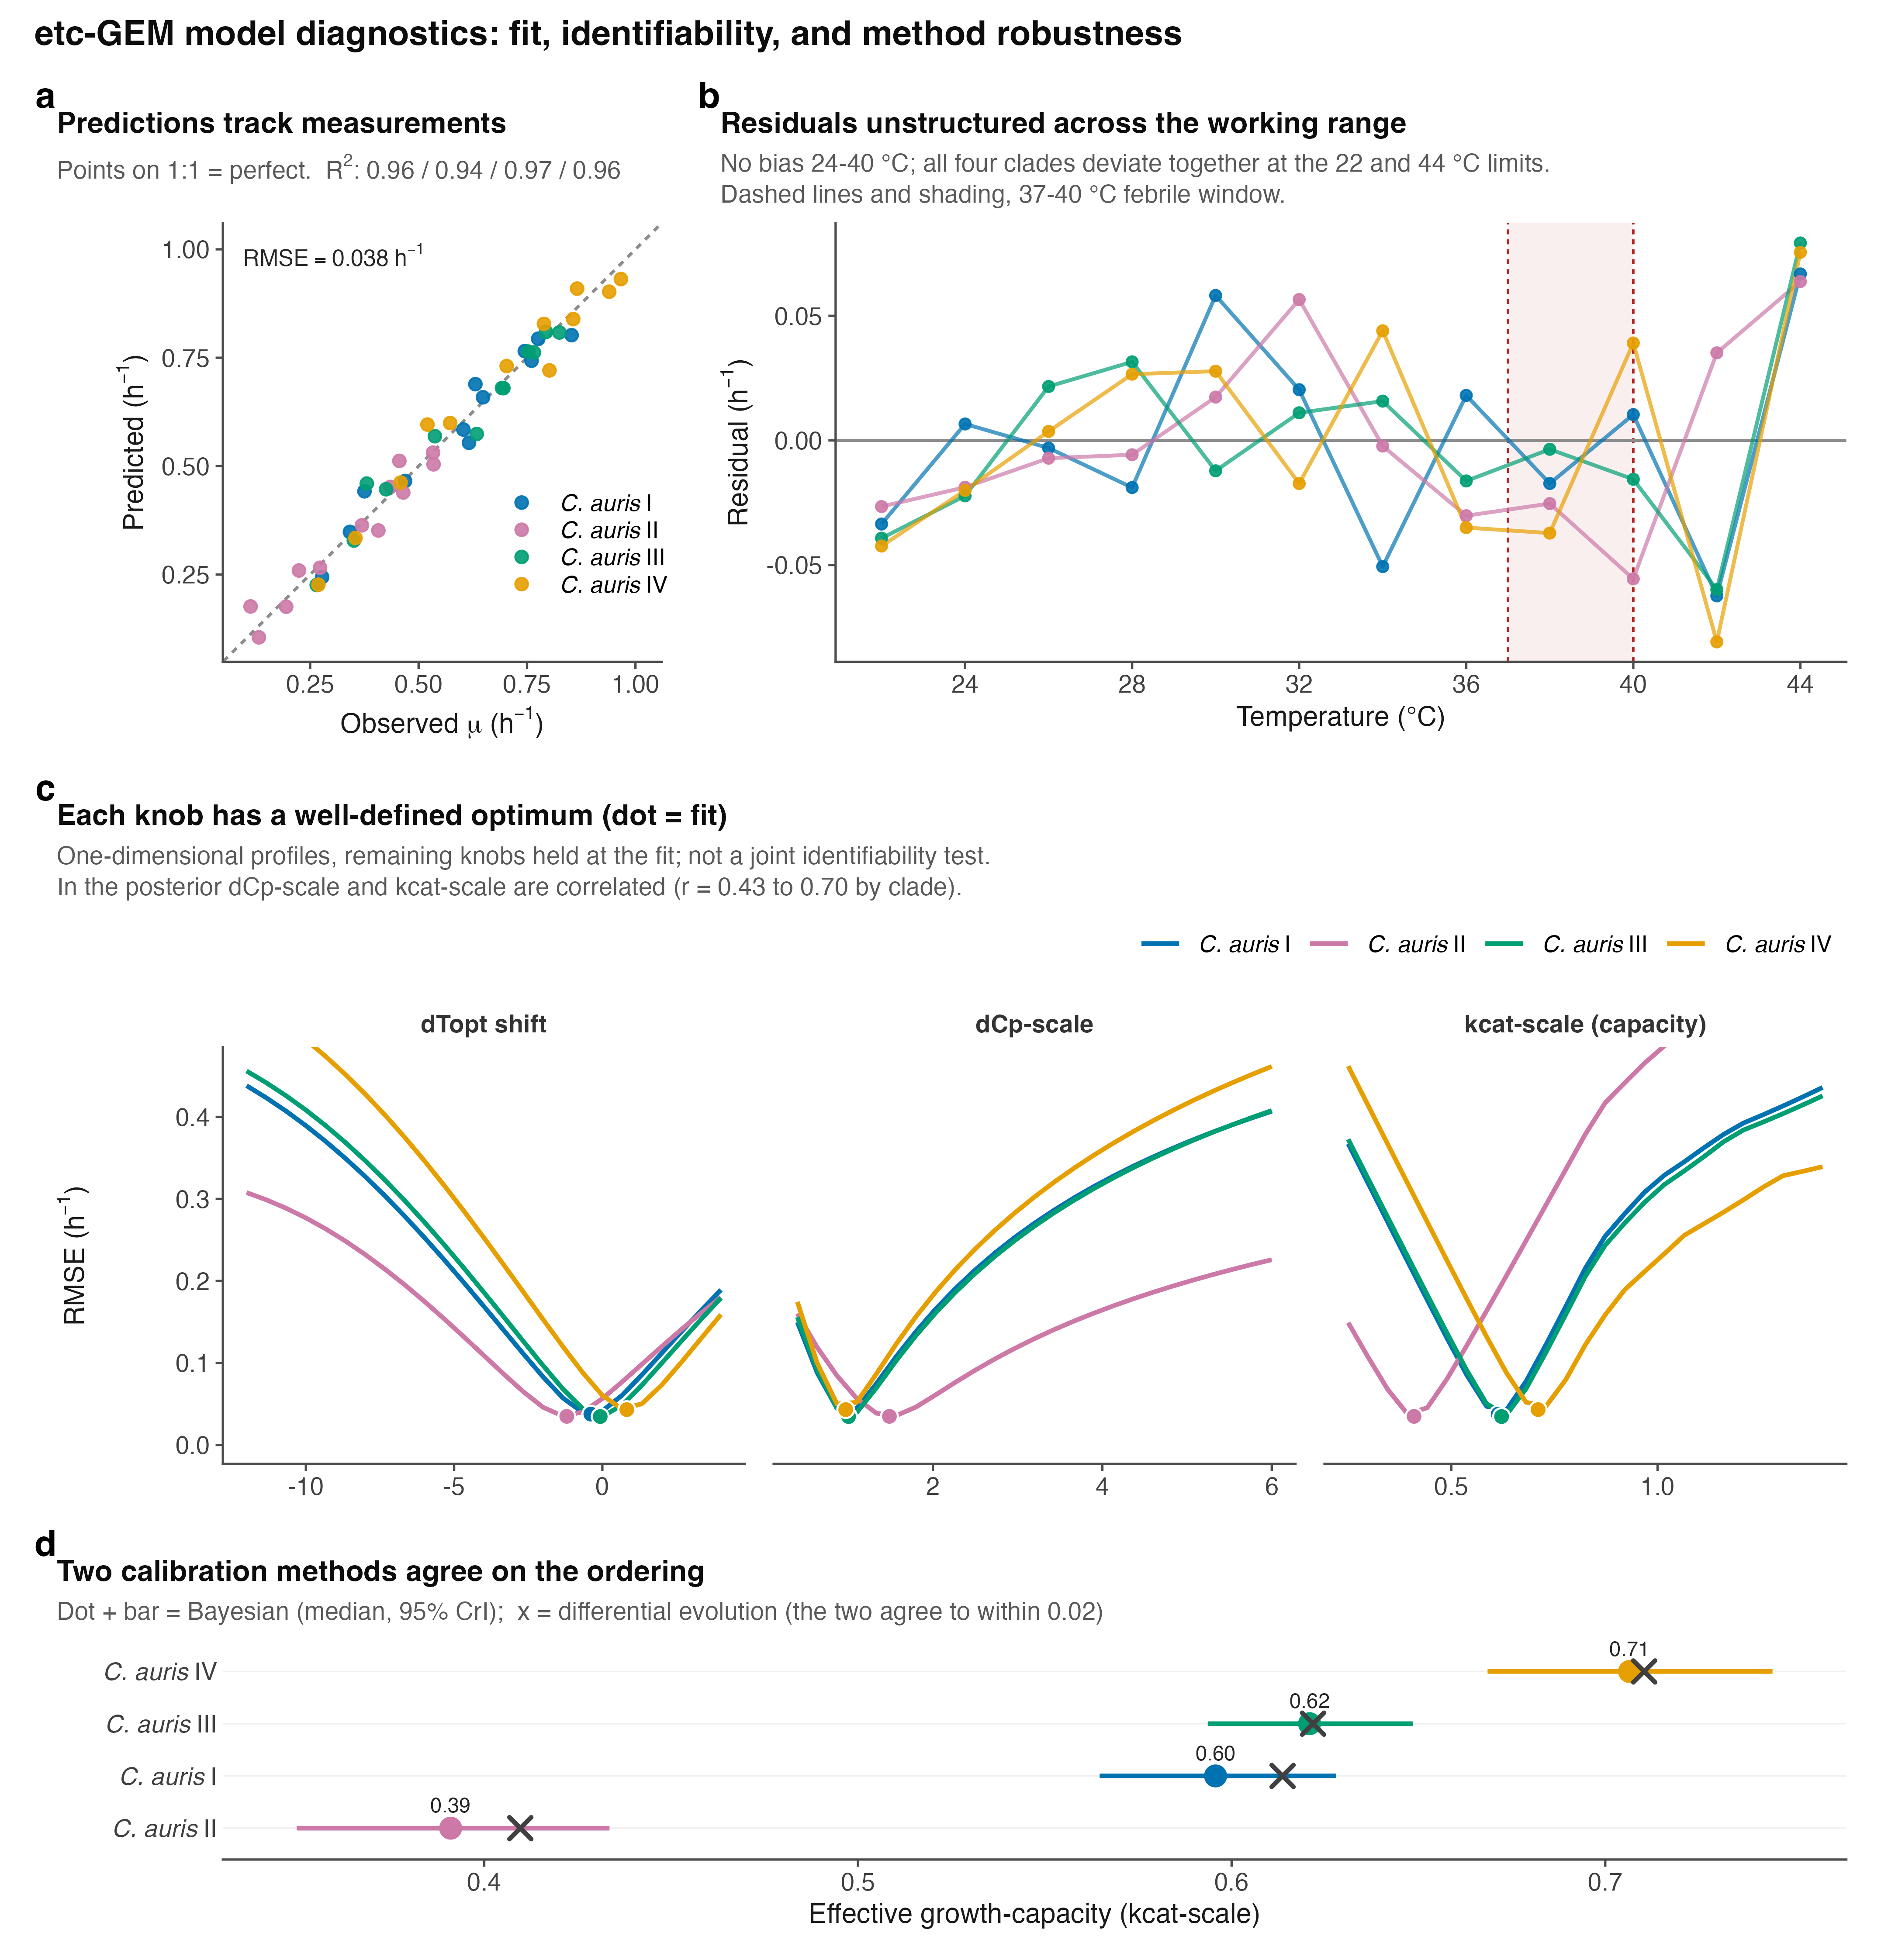
\includegraphics[width=1\linewidth,height=\textheight,keepaspectratio]{../../results/figures/manuscript/FIG_MODEL_SUPP.png}

\textbf{Supplementary Figure 2. etc-GEM model diagnostics: fit,
identifiability and method robustness.} (\textbf{a}) Predicted versus
observed growth rate for each clade under its own calibration; points on
the 1:1 line are perfect (R\textsuperscript{2} = 0.96, 0.94, 0.97 and
0.96 for Clades I-IV; overall RMSE 0.038 h\textsuperscript{-1}).
(\textbf{b}) Residuals against temperature. They are unbiased between 24
and 40 °C; at the 22 and 44 °C limits all four clades deviate together
(mean residual -0.035 and +0.071 h\textsuperscript{-1} respectively), so
the fit degrades at the edges of the assayed range. Dashed lines and
shading mark the 37-40 °C febrile window. (\textbf{c}) RMSE as each
calibration knob is swept around its optimum with the remaining knobs
held at the fit (dot). Each knob has a well-defined optimum, but these
are one-dimensional profiles and are not a joint identifiability test:
in the posterior, dCp-scale and kcat-scale are correlated (r = 0.43 to
0.70 depending on clade). (\textbf{d}) Effective growth-capacity per
clade from the two calibration methods, Bayesian median with 95\% CrI
(dot and bar) and differential evolution (x). The two agree to within
0.02 in every clade and give the same ordering.

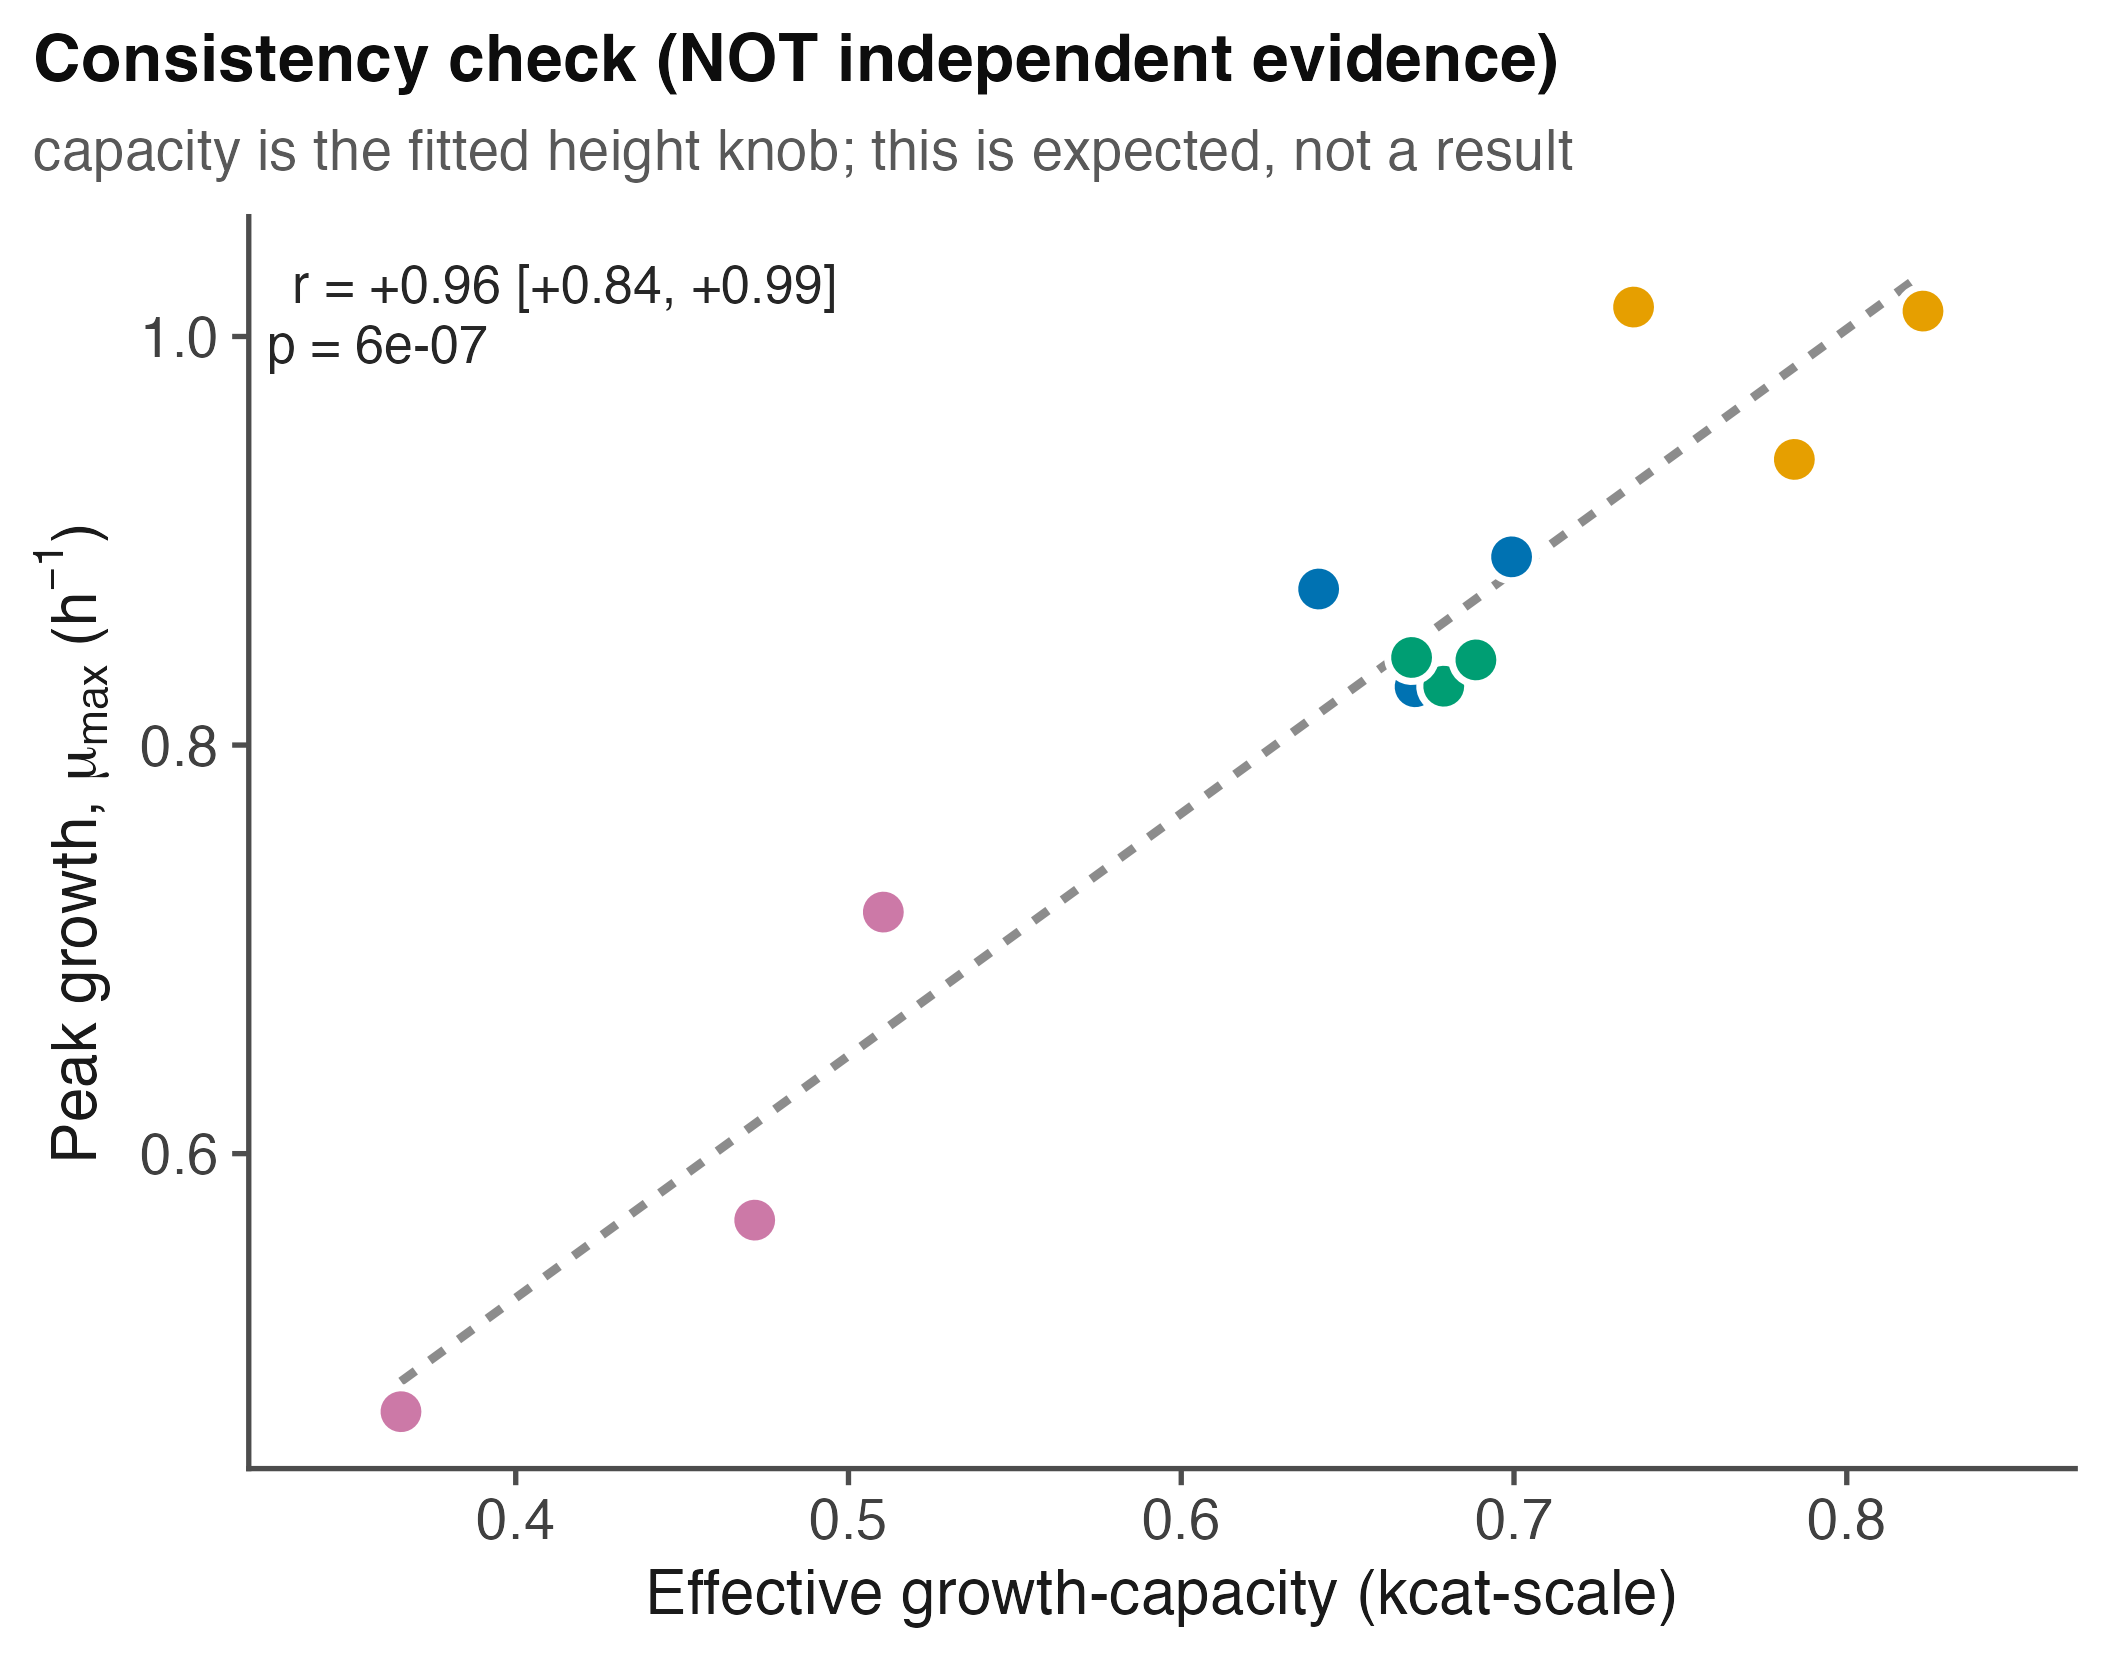
\includegraphics[width=1\linewidth,height=\textheight,keepaspectratio]{../../results/figures/manuscript/FIG_MODEL_SUPP_consistency.png}

\textbf{Supplementary Figure 3. Self-consistency check.} Effective
growth-capacity (the fitted curve-height parameter) versus measured peak
growth across the twelve isolates (r = 0.96). Because capacity scales
curve height by construction, this relationship is expected and is shown
as a consistency check, not as independent evidence; the out-of-sample
tests are in Fig. 4d-e.




\end{document}
